% ====================================================================
% COMPUTATIONAL TRACK  (concept 1 is the reference build; the rest
% follow the same template and are under construction)
% ====================================================================
\chapter{Convergence: basis order and time integration}
\label{ch:c1}
\begin{keybox}
\textbf{Key idea.} A discretization is only trustworthy if it
\emph{converges} at the rate the theory predicts. The method of
manufactured solutions (MMS) measures that rate directly: plug a known
solution into the equations, add the residual as a source, and check
that the error falls like $h^{p+1}$ in space and $\Delta t^{\,q}$ in
time.
\end{keybox}

This concept walks through the Cahn--Hilliard convergence gates that
ship with the solver: $p=1$ vs $p=2$ spatial order, and BDF1 vs BDF2
temporal order, each measured against a manufactured solution. It
connects to Physics Chapter~\ref{ch:p1} (the same brick) and to the
adaptive-stepping concept (Chapter~\ref{ch:c3}: why
variable-coefficient BDF2 matters once $\Delta t$ changes).

\section{The two kinds of error}

Every result from this simulator is wrong. The question is only
\emph{how} wrong, and whether the error shrinks --- at the rate the
theory promises --- as you refine. A finite-element discretization has
two independent discretization errors:
\begin{itemize}[nosep]
  \item a \textbf{spatial} error from representing $c(\mathbf x)$ in a
        finite basis on a mesh of size $h$; for degree-$p$ elements the
        $L^2$ error scales as $h^{p+1}$;
  \item a \textbf{temporal} error from advancing in finite steps
        $\Delta t$; for a scheme of order $q$ it scales as
        $\Delta t^{\,q}$.
\end{itemize}
The exponents $p+1$ and $q$ are \emph{predictions}. Measuring them is
the single most important correctness check in scientific computing: a
code can run, conserve mass, and look physical while quietly converging
one order too slow because a term is missing from the weak form. This
concept measures both.

\section{Spatial order: the method of manufactured solutions}

The trouble with checking a solver against a ``true'' answer is that
PDEs rarely have closed-form solutions. The \emph{method of
manufactured solutions} (MMS) turns the problem around: \emph{pick} a
smooth field, then compute what source term would make it an exact
solution, and feed that source to the solver. Now you know the exact
answer everywhere, so the error is measurable.

We manufacture the composition and the chemical potential
\emph{independently} (the cleanest choice --- it avoids taking a
Laplacian of the cubic $f'(c)$ by hand):
%
\begin{equation}
  c^\ast = \cos(\pi x)\cos(\pi y)\,e^{-t},\qquad
  \mu^\ast = \sin(\pi x)\sin(\pi y)\,e^{-t}.
\end{equation}
%
Substituting $(c^\ast,\mu^\ast)$ into the mixed Cahn--Hilliard system
\eqref{eq:ch} leaves a residual; we \emph{add it back} as two source
terms $f_c, f_m$ so the pair is an exact solution:
%
\begin{align}
  f_c &= c^\ast_t - M\,\grad^2\mu^\ast
       = -c^\ast + 2\pi^2 M\,\mu^\ast, \\
  f_m &= \mu^\ast - f'(c^\ast) + \kappa\,\grad^2 c^\ast
       = \mu^\ast - \big((c^\ast)^3 - c^\ast\big) - 2\pi^2\kappa\,c^\ast .
\end{align}
%
Because the sources are built from the exact field, everything
\emph{except} the discretization cancels: the measured $L^2$ error is
pure discretization error. We impose $c^\ast,\mu^\ast$ as strong
(Dirichlet) data on the boundary (the manufactured field is not
no-flux), then halve $h$ and watch the error fall.

\begin{keybox}
\textbf{Reading a convergence order.} If the error is
$E(h)\approx C\,h^{\,k}$, then between two meshes with $h$ and $h/2$,
$\;\log_2\!\big(E(h)/E(h/2)\big) = k$. That ratio --- the
\emph{observed order} --- is what you compare against the theoretical
$p+1$. It is far more diagnostic than any single error value: the
\emph{slope} is the physics of the method; the \emph{intercept} $C$ is
just problem-dependent.
\end{keybox}

\section{Temporal order: self-convergence}

For the time error we do not need a manufactured source. We freeze the
mesh, march the same smooth initial blend with a shrinking $\Delta t$,
and compare each run against a very fine-$\Delta t$ reference march on
the identical mesh --- so only the time error remains. Backward Euler
(\textbf{BDF1}) is first order; the two-step \textbf{BDF2} is second
order. At constant $\Delta t$, BDF2 runs its textbook coefficients
$\tfrac{3}{2}c^{n+1} = 2c^n - \tfrac12 c^{n-1} + \Delta t\,(\cdots)$;
Chapter~\ref{ch:c3} returns to what happens when $\Delta t$ is allowed
to \emph{vary} (and why the coefficients must then change).

\section{Run it}

\begin{runbox}
\textbf{Run it.}
\begin{lstlisting}
cd computational/01_convergence
python run.py            # spatial + temporal studies
\end{lstlisting}
It runs the MMS study at $p=1$ and $p=2$, the temporal study for BDF1
and BDF2, and prints the observed orders with a \code{PASS/FAIL} gate
check. Compare with \file{EXPECTED.md} and the figures below.
\end{runbox}

\begin{figure}[h]\centering
  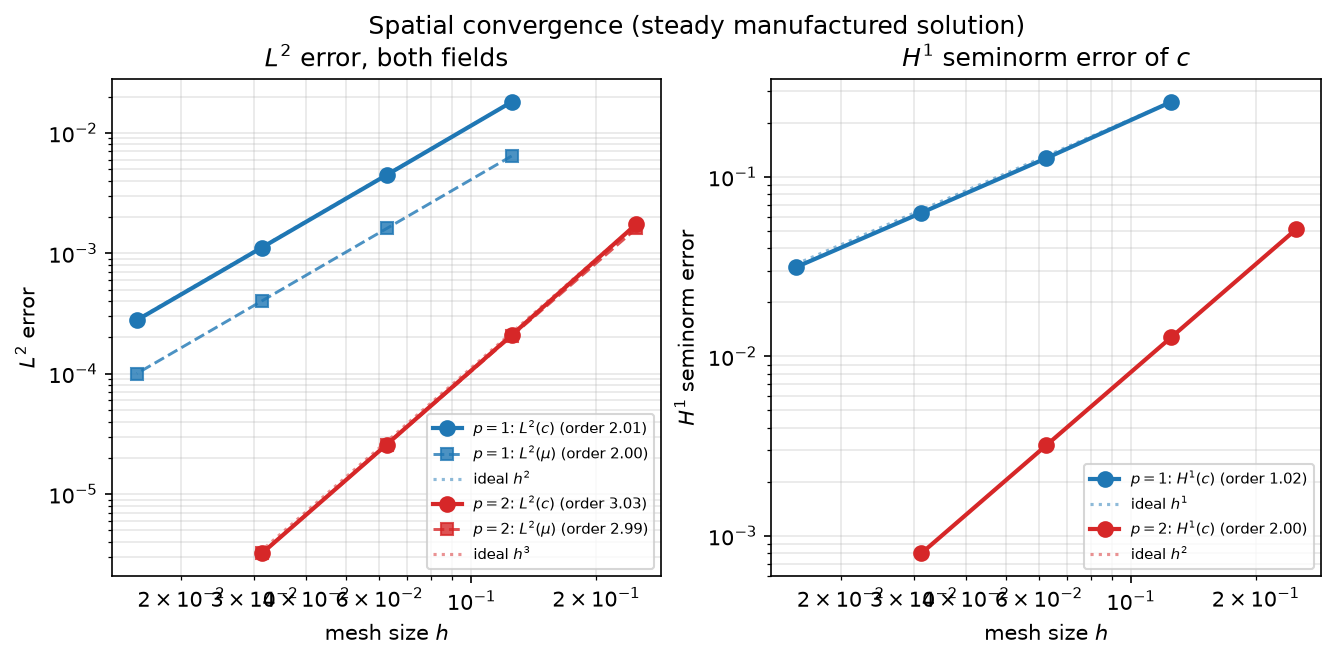
\includegraphics[width=0.86\linewidth]{figures/c1_spatial.png}
  \caption{Spatial convergence under mesh refinement. The $L^2$ error
    against the manufactured solution falls along the ideal slope
    $p{+}1$: order $\ConeSpaPoneOrder$ for $p=1$ and
    $\ConeSpaPtwoOrder$ for $p=2$ (dashed = ideal $h^{p+1}$).}
  \label{fig:c1spatial}
\end{figure}

\begin{figure}[h]\centering
  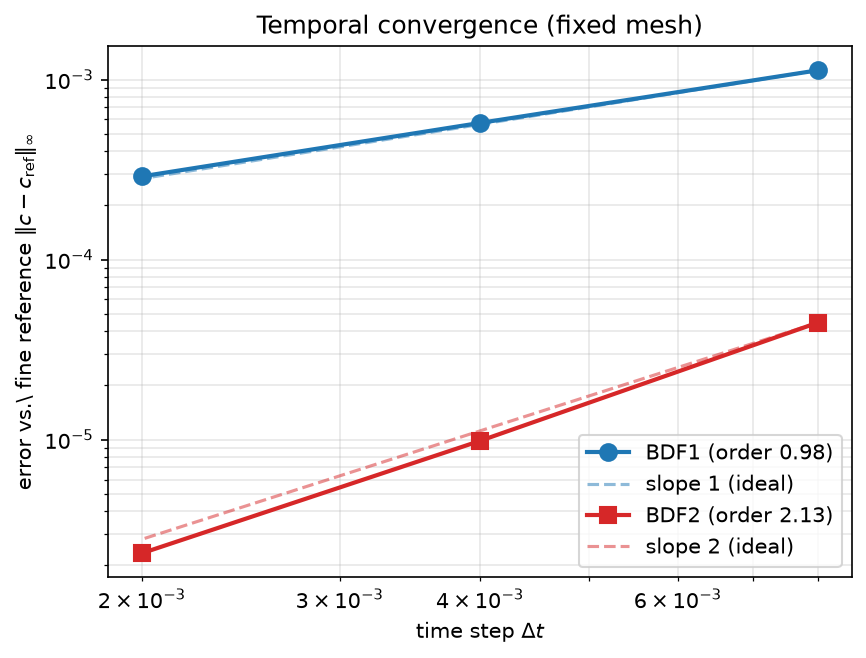
\includegraphics[width=0.86\linewidth]{figures/c1_temporal.png}
  \caption{Temporal convergence at fixed mesh. Error against a
    fine-$\Delta t$ reference march versus $\Delta t$: BDF1 tracks the
    slope-1 line (order $\ConeBdfoneOrder$), BDF2 the slope-2 line
    (order $\ConeBdftwoOrder$). At the same $\Delta t$, BDF2 is over an
    order of magnitude more accurate.}
  \label{fig:c1temporal}
\end{figure}

\begin{keybox}
\textbf{Measured self-check} (your \file{run.py} should reproduce these
to a couple of significant figures; the observed \emph{orders} are the
load-bearing quantities).
\begin{center}\small
\begin{tabular}{lccc}
\toprule
study & discretization & error (coarse $\to$ fine) & observed order \\
\midrule
spatial (MMS) & $p=1$ & \ConeSpaPoneErrCoarse\ $\to$ \ConeSpaPoneErrFine & \ConeSpaPoneOrder \\
              & $p=2$ & \ConeSpaPtwoErrCoarse\ $\to$ \ConeSpaPtwoErrFine & \ConeSpaPtwoOrder \\
\midrule
temporal      & BDF1  & \ConeBdfoneErrCoarse\ $\to$ \ConeBdfoneErrFine & \ConeBdfoneOrder \\
              & BDF2  & \ConeBdftwoErrCoarse\ $\to$ \ConeBdftwoErrFine & \ConeBdftwoOrder \\
\bottomrule
\end{tabular}
\end{center}
Expected: spatial order $p+1$ ($2$ and $3$); temporal order $1$ (BDF1)
and $2$ (BDF2).
\end{keybox}

\section{Code walk-through}

The study lives in \file{convergence.py}, which drives the production
brick \file{src/diffsim/physics/cahn\_hilliard.py} --- the same brick as
Physics Chapter~\ref{ch:p1}.

\paragraph{1. The manufactured solution and its sources.}
\begin{lstlisting}
def c_star(x, t):  return cos(pi x) cos(pi y) e^{-t}
def f_c(x, t):     return -c_star + M*2*pi^2 * mu_star   # residual, added back
\end{lstlisting}
\code{c\_star}, \code{mu\_star} are the exact fields; \code{f\_c},
\code{f\_m} are the source terms that make them exact. These are passed
to the stepper as \code{fc\_fn}, \code{fm\_fn}; the boundary data goes
in as \code{gc\_fn}, \code{gm\_fn} on the Dirichlet nodes.

\paragraph{2. The spatial sweep.}
\begin{lstlisting}
for lv in levels:                       # 4, 5, 6  (p=1)
    dm, mesh, cons = build_dm(lv, p)    # 2^lv cells per side
    st = CahnHilliardStepper(dm, M, kap, dt, order=2,
                             fc_fn=f_c, fm_fn=f_m, dirichlet=..., ...)
    for _ in range(6): c, _ = st.step()
    errs.append(l2_error(dm, cons.T @ c, lambda x: c_star(x, st.t)))
order = log2(errs[0] / errs[1])         # the observed order
\end{lstlisting}
\code{l2\_error} integrates $\|c_h - c^\ast\|$ with the same quadrature
the solver uses. The ratio of successive errors, base-2, is the order.

\paragraph{3. Temporal self-convergence.}
\begin{lstlisting}
ref = march(order=2, dt=2e-4)           # fine reference on this mesh
errs = [max|march(order, dt) - ref|  for dt in (8e-3, 4e-3, 2e-3)]
\end{lstlisting}
The reference is a high-accuracy BDF2 march; each coarse march's error
is measured against it, isolating the time error. \code{order=1}
selects BDF1, \code{order=2} selects BDF2 --- one flag in the same
constructor.

\section{Explore on your own}

\question{Add a $p=1$ level~7 ($128\times128$) point to the spatial
sweep. Does the observed order stay at $2$, or does it drift? At some
resolution the error stops being dominated by the spatial term ---
predict which term (the fixed $\Delta t$, or floating-point round-off)
takes over, and confirm it by also refining $\Delta t$.}

\question{Change the manufactured field's frequency to
$\cos(2\pi x)\cos(2\pi y)$. The error \emph{intercept} should jump (the
field is harder to resolve) while the \emph{order} stays $p+1$. Verify
both, and explain why the slope is invariant but the constant is not.}

\question{Break the solver on purpose: drop the $\kappa\,\grad^2 c$ term
from \code{f\_m} (so the source no longer matches the manufactured
field). What order do you now measure, and why is a wrong-but-nonzero
order more dangerous than an obvious crash?}

\question{Measure BDF2's temporal order at a \emph{coarser} reference
($\Delta t_{\text{ref}}=10^{-3}$ instead of $2\times10^{-4}$). At what
point does the reference stop being ``exact enough'' and the measured
order degrade? This is the self-convergence method's one pitfall ---
quantify it.}

\question{The p2 spatial study uses coarser levels (3, 4) than p1 (4, 5,
6). Why can it afford to? Count the degrees of freedom at $p{=}2$
level~4 versus $p{=}1$ level~6 and compare the two errors per DOF ---
which discretization is more accurate for the same cost here?}

\chapter{Boundary conditions, numerically}
\label{ch:c2}
\begin{keybox}
\textbf{Key idea.} A boundary condition is not an afterthought bolted
onto a solved interior --- it is baked into the weak form, and the
\emph{way} it is imposed decides what the simulation conserves. A
no-flux (natural) boundary costs nothing to impose and conserves mass
exactly; a Dirichlet boundary is imposed by replacing rows and
\emph{deliberately} breaks conservation, because it lets material cross
the boundary.
\end{keybox}

This concept shows, with measured numbers, how the two boundary
treatments the Cahn--Hilliard brick supports are imposed and what each
one costs and means. It connects to Physics Chapter~\ref{ch:p1} (whose
spinodal runs are all no-flux) and to the manufactured-solution study of
Chapter~\ref{ch:c1} (which needed Dirichlet data).

\section{Boundaries live in the weak form}

Multiply the conserved dynamics \eqref{eq:ch} by a test function $w$ and
integrate by parts:
%
\begin{equation}
  \intv w\,c_t\;+\;M\!\intv \grad w\cdot\grad\mu
  \;=\; M\!\oint_{\partial\Omega} w\,(\grad\mu\cdot\mathbf n)\,dS .
  \label{eq:weakbc}
\end{equation}
%
The entire influence of the boundary is that one surface integral. What
you do with it \emph{is} the boundary condition.

\paragraph{Natural (no-flux).}
Setting $\grad\mu\cdot\mathbf n=0$ makes the surface term vanish, and
you impose it by \emph{doing nothing} --- simply omit the integral. This
is why it is called \emph{natural}: it is the condition the weak form
adopts on its own. Physically it is a zero-flux wall: no mass crosses
$\partial\Omega$, so total mass $\intv c\,dV$ is conserved to solver
tolerance. Every spinodal run in Physics Chapter~\ref{ch:p1} is a
no-flux run, which is why its mass drift was machine epsilon.

\paragraph{Dirichlet (fixed value).}
To hold the boundary composition at a prescribed $g$ we cannot use the
surface term --- we \emph{replace} the boundary rows of the assembled
system with the identity, $\;A_{ii}\!\leftarrow\!1$, right-hand side
$\leftarrow g - x_i$ (the Newton-increment form). This pins $(c,\mu)$ at
those nodes exactly. It is the treatment the manufactured-solution study
of Chapter~\ref{ch:c1} needed (the exact field is not no-flux), and it
models a composition held fixed at a contact. Crucially, a pinned
boundary \emph{is} a reservoir: whatever flux is needed to maintain the
value flows freely, so mass is \textbf{not} conserved --- by design.

\begin{keybox}
\textbf{A boundary condition changes what you conserve.} No-flux
conserves mass because it forbids boundary flux. Dirichlet abandons
conservation because it fixes a value and lets flux adjust. Neither is
``more correct'' --- they model different physical situations (a sealed
domain vs.\ a contact held at a set composition). Choosing wrong gives a
plausible-looking but physically wrong answer.
\end{keybox}

\paragraph{A third kind: wall free energy.}
A real thin film often \emph{wets} its substrate: one component prefers
the wall. That is a surface free energy $\oint g_s(c)\,dS$ added to
\eqref{eq:F}, which makes the natural flux \emph{nonzero} (a Robin-type
wetting condition) rather than pinning a value. It is genuine physics,
but it lives in the multiphase film brick, not this binary
Cahn--Hilliard brick (see \file{docs/dev/2026-07-13-m5-device-assembly.md},
the A2 wall term); we name it here for completeness and use it in the
device track. This tutorial measures the two treatments the binary brick
implements.

\section{Run it}

\begin{runbox}
\textbf{Run it.}
\begin{lstlisting}
cd computational/02_boundary_conditions
python run.py            # both boundary treatments, compared
\end{lstlisting}
It marches the \emph{identical} spinodal blend (same fixed seed) twice
--- once no-flux, once with every box edge pinned to $c=\CtwoWall$ ---
and prints the mass drift and boundary layer of each. Compare with
\file{EXPECTED.md} and Fig.~\ref{fig:c2fields}--\ref{fig:c2mass}.
\end{runbox}

\begin{figure}[h]\centering
  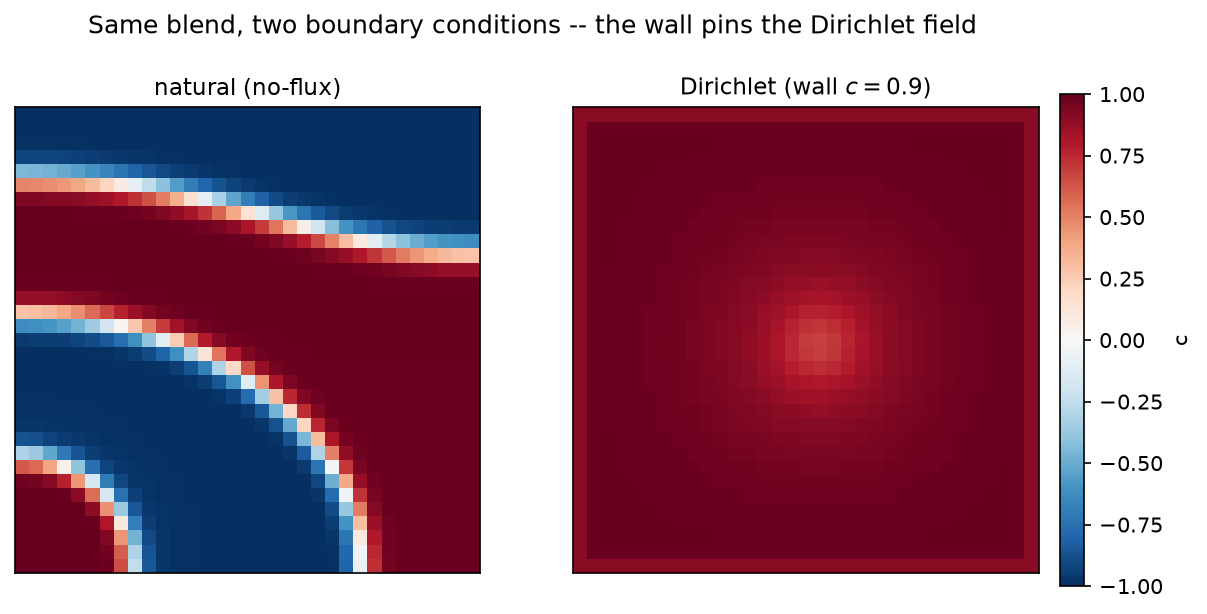
\includegraphics[width=0.92\linewidth]{figures/c2_fields.png}
  \caption{The same blend under the two boundary conditions. Left:
    no-flux --- domains meet the wall freely. Right: Dirichlet ---
    the edge is pinned to $c=\CtwoWall$ and that phase is drawn to the
    boundary, reorganizing the morphology. The measured field
    difference is $\CtwoFieldDiff$ (the full order-parameter range).}
  \label{fig:c2fields}
\end{figure}

\begin{figure}[h]\centering
  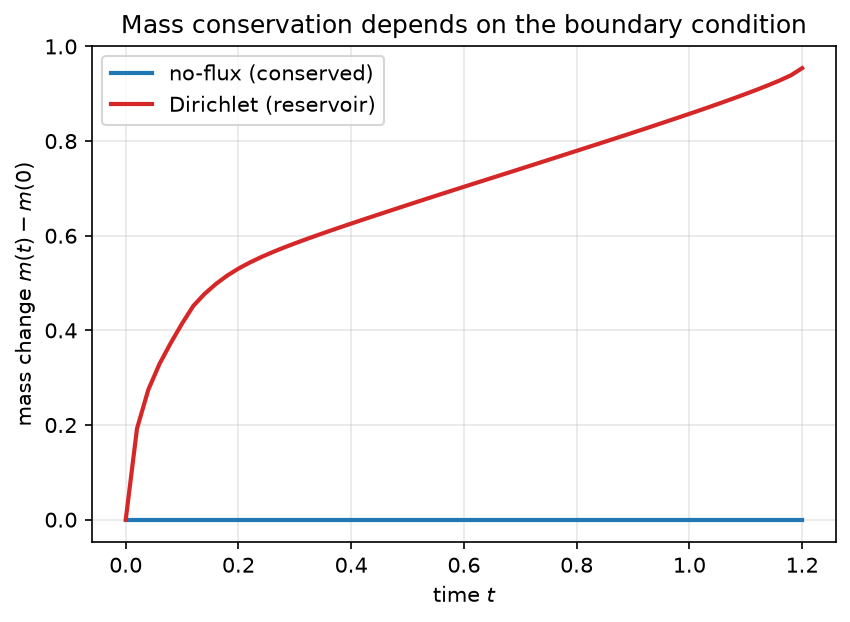
\includegraphics[width=0.7\linewidth]{figures/c2_mass.png}
  \caption{Mass change $m(t)-m(0)$. The no-flux wall conserves mass to
    machine precision (flat at zero); the Dirichlet wall acts as a
    reservoir and draws material in ($\Delta m\approx\CtwoDirMassDrift$).}
  \label{fig:c2mass}
\end{figure}

\begin{keybox}
\textbf{Measured self-check} (fixed seed in \file{bc.py}; field values
are seed-dependent, the conservation/pinning contrast is not).
\begin{center}\small
\begin{tabular}{lcc}
\toprule
 & natural (no-flux) & Dirichlet ($c=\CtwoWall$) \\
\midrule
mass drift $|\Delta m|$ & \CtwoNfMassDrift & \CtwoDirMassDrift \\
edge composition        & \CtwoNfEdge\ (free) & \CtwoDirEdge\ (pinned) \\
field difference max$|c_{\text{nf}}-c_{\text{dir}}|$ & \multicolumn{2}{c}{\CtwoFieldDiff} \\
\bottomrule
\end{tabular}
\end{center}
\end{keybox}

\section{Code walk-through}

The comparison lives in \file{bc.py}, driving the same production brick.

\paragraph{Selecting the boundary.}
\begin{lstlisting}
# natural: pass nothing -- the default weak form is no-flux
st = CahnHilliardStepper(dm, M, kap, dt, order=1)

# Dirichlet: pass the boundary node indices + the data functions
st = CahnHilliardStepper(dm, M, kap, dt, order=1, dirichlet=bidx,
                         gc_fn=lambda x,t: wall, gm_fn=lambda x,t: 0)
\end{lstlisting}
\code{boundary\_free\_nodes} finds the box-edge nodes; \code{gc\_fn},
\code{gm\_fn} supply the pinned $(c,\mu)$ values. The natural case needs
no argument at all --- the load-bearing point of the concept.

\paragraph{Measuring the effect.}
\begin{lstlisting}
m0 = mass(st, st.hist[0])
for _ in range(steps): c, _ = st.step()
drift = abs(mass(st, c) - m0)          # ~1e-16 no-flux; ~0.95 Dirichlet
\end{lstlisting}
\code{mass} integrates $\intv c\,dV$ with the solver's own quadrature ---
the same conservation diagnostic as Physics P1. Running both modes from
the identical seeded initial field isolates the boundary's effect in the
field difference.

\section{Explore on your own}

\question{Sweep the Dirichlet wall value $g\in\{-0.9,0,+0.9\}$. Predict
the sign and rough size of $\Delta m$ for each before running, then
check. For which $g$ is mass \emph{approximately} conserved, and is that
a coincidence of the initial mean?}

\question{Pin only \emph{two} opposite edges (left/right) instead of all
four, leaving top/bottom no-flux. How does the boundary layer and the
mass drift change? This mixed condition is common in device geometries
(contacts on two sides, sealed on the others).}

\question{The no-flux mass drift is $\sim10^{-16}$ --- machine epsilon,
not solver tolerance. Refine the mesh one level and re-measure: does the
drift grow with the number of nodes (accumulated round-off) or stay at
machine level? What does that tell you about how conservation is
enforced here?}

\question{Under Dirichlet, the boundary $\mu$ is pinned to $0$. Is that
physical? Argue what $\mu$ at a composition-pinned contact \emph{should}
be, and why pinning both $c$ and $\mu$ (as this brick does) is a
modelling choice, not a law. What would a $c$-only Dirichlet require of
the solver?}

\question{Estimate the ``cost'' of each boundary condition: count how
many rows the Dirichlet case replaces versus the interior, and argue why
the natural condition is not only physically distinct but computationally
free.}

\chapter{Spatial and temporal adaptivity}
\label{ch:c3}
\begin{keybox}
\textbf{Key idea.} Resolution should follow the physics. In space,
\emph{octree refinement} puts small elements only where the field is
sharp (the interfaces) and leaves the bulk coarse. In time, an
\emph{LTE-controlled} step ladder shrinks $\Delta t$ during the violent
onset and grows it through slow coarsening --- but growing $\Delta t$
safely forces BDF2 to carry its \emph{variable-coefficient} form, or its
order silently collapses.
\end{keybox}

This concept measures both adaptivities on the Cahn--Hilliard brick. It
builds directly on the convergence study (Chapter~\ref{ch:c1}: the BDF2
order that adaptivity must preserve) and enables the long phase-field
horizons the physics track needs.

\emph{Under construction --- octree refinement and the LTE/PI step
controller.}
\chapter{The solver ecosystem}
\emph{Under construction --- direct (cuDSS) vs the \texttt{blockch}
block preconditioner vs matrix-free, and when each wins (with the
measured tables).}
\chapter{Two dimensions versus three}
\emph{Under construction --- cost, memory, and the assembly/solve story
at scale.}
